\documentclass[conference]{IEEEtran}
\IEEEoverridecommandlockouts
% The preceding line is only needed to identify funding in the first footnote. If that is unneeded, please comment it out.
\usepackage{cite}
\usepackage{amsmath,amssymb,amsfonts}
\usepackage{algorithmic}
\usepackage{graphicx}
\usepackage{textcomp}
\usepackage{xcolor}
\usepackage{listings}
\def\BibTeX{{\rm B\kern-.05em{\sc i\kern-.025em b}\kern-.08em
    T\kern-.1667em\lower.7ex\hbox{E}\kern-.125emX}}
\lstset{language=c++, frame=single, numbers=left, xleftmargin=2em, framexleftmargin=2em, breaklines=true, basicstyle=\scriptsize}
\graphicspath{ {./images/} }
\begin{document}

\title{Parallelizing Sorting Algorithms}

\author{\IEEEauthorblockN{Kevin Alfonso}
\IEEEauthorblockA{\textit{Computer Science, UCF} \\
\textit{Parallel - Group 1}\\
Orlando, Florida \\
kevfonso@knights.ucf.edu}
\and
\IEEEauthorblockN{Gabriella On-Cuen }
\IEEEauthorblockA{\textit{Computer Science, UCF} \\
\textit{Parallel - Group 1}\\
Orlando, Florida \\
Gabriella2024@knights.ucf.edu}
\and
\IEEEauthorblockN{Faiz Ahmed}
\IEEEauthorblockA{\textit{Computer Science, UCF} \\
\textit{Parallel - Group 1}\\
Orlando, Florida \\
faiz@knights.ucf.edu}
\and
\IEEEauthorblockN{Raciel Antela Pardo}
\IEEEauthorblockA{\textit{Computer Science, UCF} \\
\textit{Parallel - Group 1}\\
Orlando, Florida \\
raciel@knights.ucf.edu}
\and
\IEEEauthorblockN{Isaac Munshi}
\IEEEauthorblockA{\textit{Computer Science, UCF} \\
\textit{Parallel - Group 1}\\
Orlando, Florida \\
isaac.p.munshi@knights.ucf.edu}
}

\maketitle

\begin{abstract}
% Common sorting algorithms were implemented in parallel to explore the differences in run-time and efficiency between the multi-threaded version of the algorithm and the regular one. The algorithms tested in this experiment were bubble sort, merge sort, and radix sort. It has been found that parallelizing sorting algorithms does in fact decrease the run times significantly in some cases such as bubble sort while more moderately in others such as merge sort and radix sort. 
% old version ^
Common sorting algorithms were implemented in parallel to explore the differences in run-time and efficiency between the multi-threaded implementations of the algorithms and the original linear versions. The algorithms tested in this experiment were bubble sort, merge sort, and radix sort. It has been found that parallelizing sorting algorithms does in fact improve run-time and efficiency. In some algorithms such as bubble sort, the run-times were reduced significantly, while in others such as merge sort and radix sort, the improvements were moderate but still a notable increase.

\end{abstract}

\section{Introduction}
Sorting is used everywhere in computer science, from student projects to enterprise-level software. Oftentimes, this deals with large amounts of data which leads to the sorting taking longer. By rewriting popular sorting algorithms to take advantage of parallelism and multithreading in a clever way, we can reduce the time it takes to sort large amounts of data at the cost of increased computing power, which is a worthwhile trade due to computers getting more powerful since the days the original sorting algorithms were written and implemented. We have rewritten Merge Sort, Radix Sort, and Bubble Sort. 

We expected for each sort to take less time, at least when it comes to large arrays. We also expected for CPU usage to increase compared to the normal sorting algorithms.

% \section{Problem Statement}
% For this project we have rewritten bubble sort, merge sort, and radix sort in C++. 

% \section{Related Work}
% N/A

\section{Technique/Methodology}
We wrote these revised sorting algorithms in C++. We used std::thread to create parallel threads that work on distinct parts of the data simultaneously. Additionally, we used techniques such as lock-free data structures and atomic operations to avoid any race conditions or other synchronization issues that may arise during the parallelization process; this includes the usage of vectors of threads to improve concurrent thread safety and performance as opposed to arrays.

We implemented the normal sorting algorithms and then parallelized them. We tested each sorting algorithm with 1 (not parallel), 2, 4, and 8 threads. We had each thread complete its own sorting work and then merged them together at the end, which typically improves the run-time when compared to doing the same work with only 1 thread.

\subsection{Bubble Sort}
For our concurrent bubble sort, we first figure out how big each chunk of the array should be based on the array size and number of threads. If the array size is evenly divisible by the number of threads, then the threads handle the same size chunk. Otherwise, the last chunk handles the smaller remainder of data and likely finishes faster. Afterwards, we assign each thread its respective chunk and make it bubble sort it. We join the threads to ensure they are all finished sorting, and then proceed to the final merge step to join together all the chunks of data. This merge is similar to the merge step in merge sort, in that it merges adjacent chunks together, doubling in size every iteration.

% We could not find a way to avoid merging the arrays at the end without sacrificing the correctness of the algorithm or its performance. Running bubble sort for the already sorted chunks would significantly slow down the algorithm. Merging, on the other hand, is much faster since we can take advantage of the already sorted data in the chunks. In practice, this means that concurrent bubble sort is a hybrid implementation of bubble sort and merge sort.

% \begin{figure}[htbp]
\begin{lstlisting}
template<class T>
void concurrentBubbleSort(T arr[], int n, int numThreads) {
    vector<thread> threads;

    int chunk_size = (int)floor(n / numThreads);

    for (int i = 0; i < numThreads - 1; i++) {
        int start = i * chunk_size;
        int end = start + chunk_size;
        threads.emplace_back(bubbleSort<T>, ref(arr), start, end);
    }
    threads.emplace_back(bubbleSort<T>, ref(arr), (numThreads - 1) * chunk_size, n);

    for (auto &thread: threads) {
        thread.join();
    }

    for (int size = chunk_size; size < n; size *= 2) {
        for (int i = 0; i < n - size; i += 2 * size) {
            int left = i;
            int mid = i + size - 1;
            int right = min(i + 2 * size - 1, n - 1);
            merge(arr, left, mid, right);
        }
    }
};
\end{lstlisting}
% \caption{Concurrent Implementation of Bubble Sort}
% \label{fig}
% \end{figure}

\subsection{Merge Sort}
Here is part of our implementation for our concurrent Merge Sort. Just like in the normal linear merge sort, we split our array in half recursively. However, we also assign each half to a thread until we run out of threads. Once we run out of threads, we continue splitting the array like normal, then sort, and finally merge. This approach has no waiting or locks and avoids contention. Even though a thread has two sub-threads inside of it, the threads will never fight over accessing data as each thread has its own subset of data and the thread dies after finishing it's job and it passes the array to the parent-thread. Thus, we have successfully parallelized the merge sort function.

% \begin{figure}[htbp]
\begin{lstlisting}
template <class T>
void concurrentMergeSort(T arr[], int start, int end, int numThreads) {
    if (start < end) {
        int mid = (start + end) / 2;
        
        if (numThreads > 1) {
            vector<thread> threads(2);

            int numThreadsLeft = numThreads / 2;
            int numThreadsRight = numThreads - numThreadsLeft;

            threads[0] = thread(concurrentMergeSort<T>, arr, start, mid, numThreadsLeft);
            threads[1] = thread(concurrentMergeSort<T>, arr, mid + 1, end, numThreadsRight);
            
            for (auto& thread : threads) {
                thread.join();
            }
        } else {
            concurrentMergeSort(arr, start, mid, 1);
            concurrentMergeSort(arr, mid + 1, end, 1);
        }

        merge(arr, start, mid, end);
    }
}
\end{lstlisting}
% \caption{Concurrent Implementation of Merge Sort}
% \label{fig}
% \end{figure}

\subsection{Radix Sort}
Our concurrent radix sort is implemented extremely similarly to the concurrent bubble sort. We split the array into chunks based on the array size and number of threads, assign each thread to radix sort its respective chunk, join the threads, then merge all the chunks together.

% \begin{figure}[htbp]
\begin{lstlisting}
void concurrentRadixSort(int arr[], int n, int numThreads)
{
    vector<thread> threads;
    
    int chunk_size = (int)floor(n / numThreads);

    for (int i = 0; i < numThreads - 1; i++) {
        int start = i * chunk_size;
        int end = min(start + chunk_size, n);
        threads.emplace_back(radixSort, ref(arr), start, end);
    }
    threads.emplace_back(radixSort, ref(arr), (numThreads - 1) * chunk_size, n);
    
    for (auto &thread: threads) {
        thread.join();
    }

    for (int size = chunk_size; size < n; size *= 2) {
        for (int i = 0; i < n - size; i += 2 * size) {
            int left = i;
            int mid = i + size - 1;
            int right = min(i + 2 * size - 1, n - 1);
            merge(arr, left, mid, right);
        }
    }
}
\end{lstlisting}
% \caption{Concurrent Implementation of Radix Sort}
% \label{fig}
% \end{figure}

\subsection{Insertion Sort}
Our concurrent insertion sort is implemented extremely similarly to the concurrent bubble sort and radix sort. We split the array into chunks based on the array size and number of threads, assign each thread to insertion sort its respective chunk, join the threads, then merge all the chunks together.

% \begin{figure}[htbp]
\begin{lstlisting}
void concurrentInsertionSort(int arr[], int n, int num_threads) {
    vector<thread> threads;
    int chunk_size = n / num_threads;
    int start = 0;
    int end = chunk_size;
    for (int i = 0; i < num_threads; i++) {
        threads.emplace_back(insertionSort, ref(arr), start, end - 1);
        start = end;
        end = min(end + chunk_size, n);
    }

    for (auto &thread : threads) {
        thread.join();
    }
    for (int i = 1; i < num_threads; i++) {
        int mid = i * chunk_size - 1;
        int right = min((i + 1) * chunk_size - 1, n - 1);
        merge(arr, 0, mid, right);
    }
}
\end{lstlisting}
% \caption{Concurrent Implementation of Radix Sort}
% \label{fig}
% \end{figure}

\section{Evaluation}
To evaluate our sorts, we outputted all the data collected for each run (sort name, array size, time taken, CPU usage, and number of threads used) into a table through standard output for easy viewing by anyone who runs the code, as well as a CSV file to make charts and plots from the data in a Python script, allowing us to easier visualize relationships between all the variables.

\subsection{Bubble Sort}
Bubble sort was the golden child of showing relationships in our data. It very clearly shows that at some point between 100 and 1000 for the array size, bubble sort benefits more from multi-threading through time saving than it wastes time from the thread creation and management overhead.
As for the CPU usage, it shows in an almost exact perfect relationship that multithreading puts more strain on the CPU compared to sequential programming (doubling threads means doubling CPU usage percent). However, as mentioned in the introduction, this is often worth it due to constantly improving computing power mixed with a need for quickly sorted data.
\includegraphics[width=3.5in]{BubbleSortTimeTaken.png}
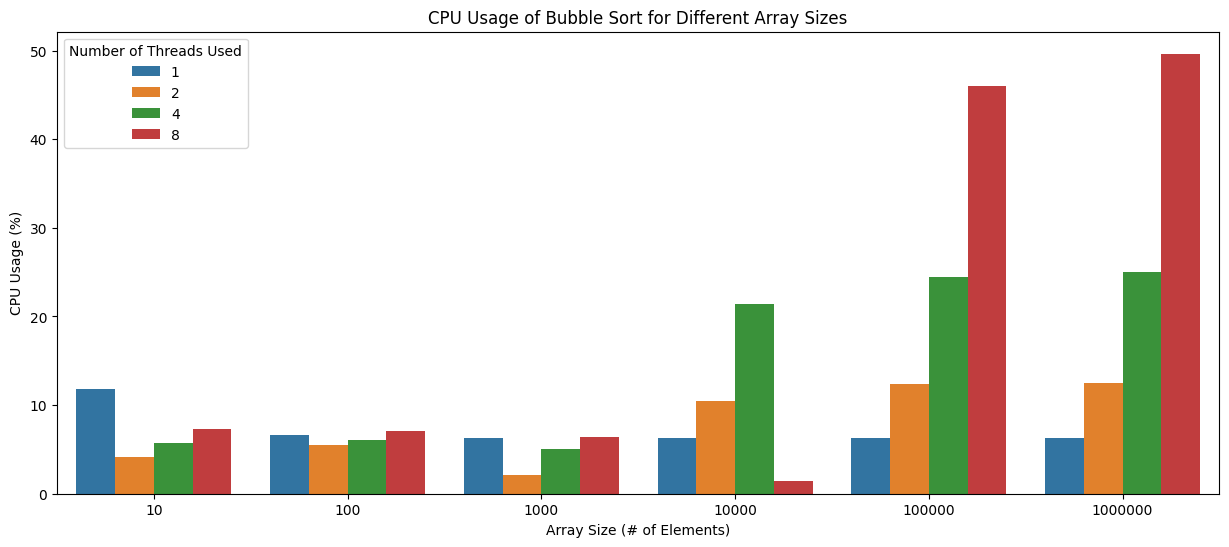
\includegraphics[width=3.5in]{BubbleSortCPUUsage.png}

\subsection{Merge Sort}
Merge sort is so fast compared to bubble sort that the point for when multi-threading becomes beneficial is between 1000 and 10000 for the array size. Its improved run-time also means it has less room for improvement as we double the amount of threads, especially compared to bubble sort.
Merge Sort's CPU usage relationship is slightly less apparent than bubble sort's, but it can be seen that certain array sizes indeed raise CPU usage as thread count is increasing, pointing more towards the measurable cost of thread overhead.
\includegraphics[width=3.5in]{MergeSortTimeTaken.png}
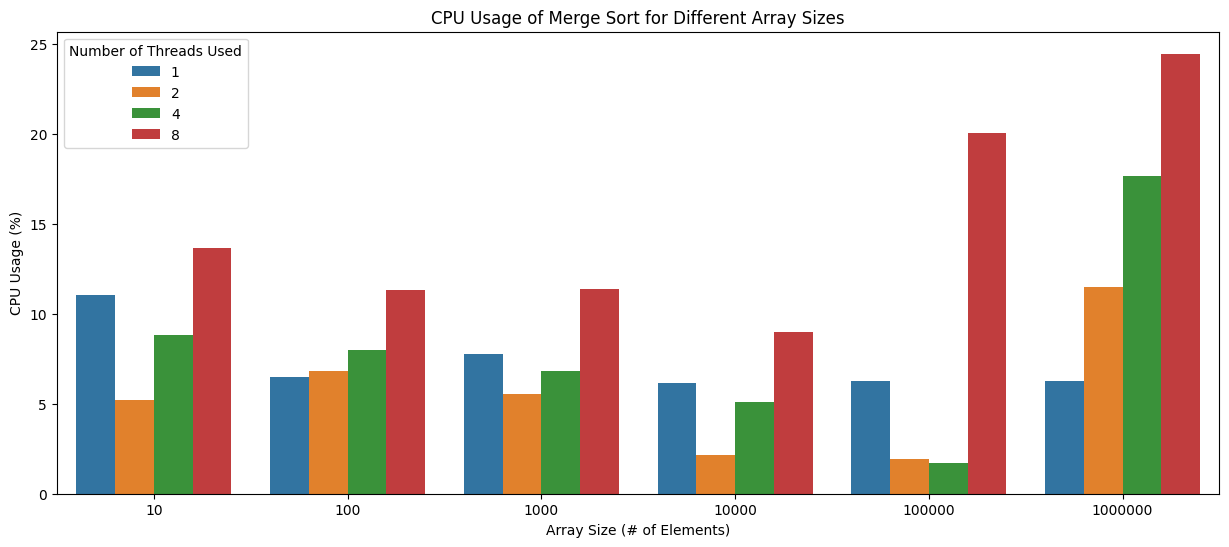
\includegraphics[width=3.5in]{MergeSortCPUUsage.png}

\subsection{Radix Sort}
Radix sort benefited the least from an increasing number of threads. Our results show that the best approach is to use 4 threads when your array is 10,000 elements or more. 
For datasets of size 10,000 or more, run-time was improved from 1 to 2 threads, the improvement from 2 to 4 threads was small, and there was little to no improvement from 4 to 8 threads. In fact, the 8-thread approach used significantly more CPU resources making it an over-all worse approach than the 4-thread approach! Also interestingly is that in almost every array size, the CPU usage for 4 threads was smaller than the 2-thread approach.
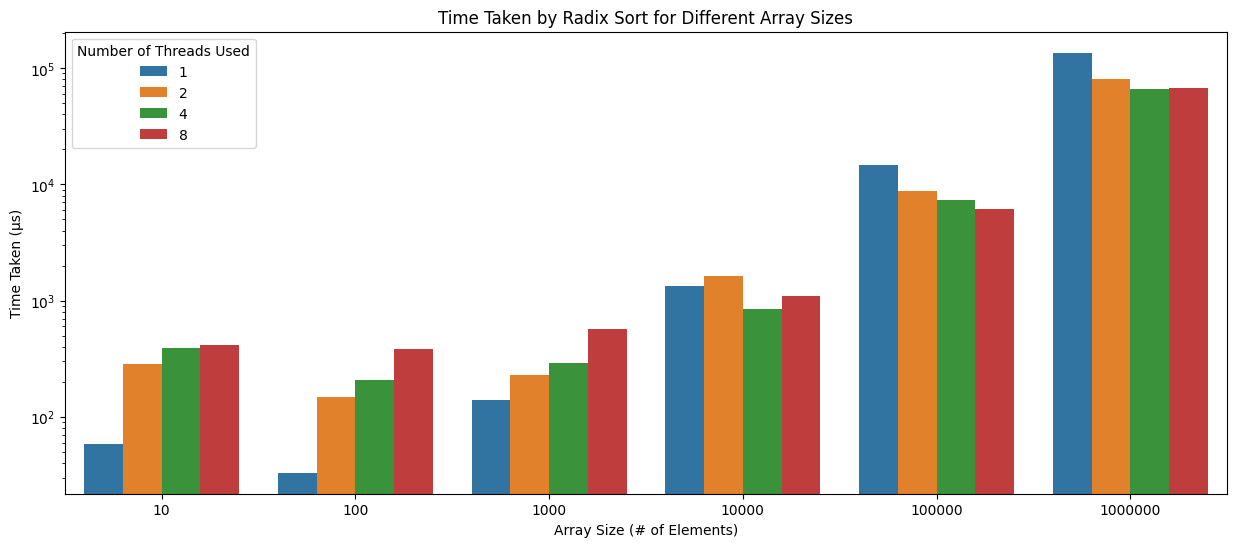
\includegraphics[width=3.5in]{RadixSortTimeTaken.png}
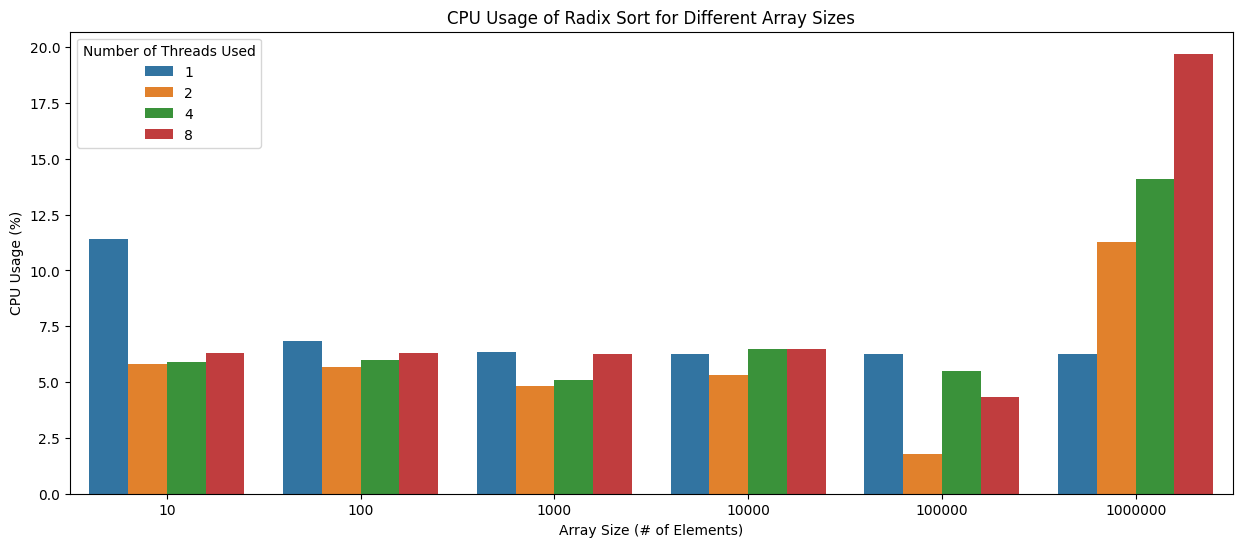
\includegraphics[width=3.5in]{RadixSortCPUUsage.png}

\subsection{Insertion Sort}
Insertion sort showed noticeable benefits when multi-threading, likely due to the fact that its runtime is on the slower side. Like bubble sort, it very clearly shows that at some point between 100 and 1000 for the array size, insertion sort benefits more from multi-threading through time saving than it wastes time from the thread creation and management overhead. At the higher array sizes, multithreading leads to higher CPU usage. At higher array sizes, there is a perfect correlation between array size and CPU usage. If you double the array size, you double the CPU usage.

\section{Discussion}
The implementations our team designed showed great results, but there are many ways to implement concurrency in sorting algorithms. For example, researchers could try implementing concurrency in sorts without needing a merge step at the end by having the merge be done "along the way" as the sort is being completed, and that could possibly speed it up over one large merge step. In the future, other researchers can take different approaches to parallelizing the sorting methods addressed in our paper and compare results. There are always more ways to assign jobs to threads. Or, they can take our research and apply it to new methods we have not covered.

\section{Conclusion}
Overall, our data appears to confirm our original hypothesis that implementing these common sorts with multi-threading improves time taken for that sort to complete at the cost of increased CPU usage of the system. However, this is only worth it for larger array sizes (the specific size depends on the type of sort and specifications of the system doing the sorting), so be sure to do some testing of your own.

\end{document}
